\documentclass{article}
\usepackage{iclr2026_conference,times}
\input{math_commands.tex}
\usepackage{graphicx}
\usepackage{booktabs}
\usepackage{hyperref}
\usepackage{url}

\title{Where Do Bits Matter in World Models?\\Evidence for a 4-bit Transition in DINO-WM Planning}
\author{}

\begin{document}
\maketitle
\lhead{Under review as a workshop paper at ICLR 2026 (ES-Reasoning)}

\begin{abstract}
Efficient spatial reasoning systems need world models that remain reliable under strict compression budgets.
We study weight-only quantization in DINO-WM planning on Wall and ask whether performance is controlled only by bitwidth, or also by \emph{where} precision is preserved.
We combine a pilot ten-variant sweep with a larger paired-goal transition study that evaluates two planner budgets, 39 total runs, and 390 paired episodes.
Across both runs, we observe a consistent three-regime pattern: 8-bit variants match FP16, 3-bit variants collapse, and 4-bit is a transition regime where allocation matters.
Under paired evaluation, mixed INT4 (encoder FP16, predictor INT4) outperforms uniform INT4 by +0.20 success at budget bA (95\% bootstrap CI [0.00, 0.40], $n=30$ paired episodes) and by +0.30 at budget bB (CI [0.00, 0.55], $n=20$).
Mechanistic diagnostics show strong negative rank correlation between embedding divergence and planning success, suggesting that representation degradation is a plausible failure pathway near the low-bit frontier.
These results motivate module-aware precision allocation as a concrete direction for efficient world-model planning.
\end{abstract}

\section{Introduction}
World-model planning has become a central approach for efficient decision making in visuomotor control, with strong results from latent-dynamics models and pretrained visual features \citep{hafner2023dreamerv3,zhou2024dinowm,oquab2023dinov2}.
At deployment time, however, these systems are increasingly constrained by memory and latency budgets.
Low-bit post-training quantization is therefore attractive, but broad evidence shows that robustness often degrades sharply in ultra-low-bit regimes \citep{liu2025lowbitmodelquantizationdeep}.
Recent world-model-specific evidence also suggests that quantization sensitivity can be module dependent rather than uniform \citep{fu2026quantwm}.

This paper targets a precise workshop question: in planning with world models, is performance determined mainly by total bitwidth, or by bit allocation across representation and dynamics modules?
We study this question in DINO-WM by comparing uniform quantization (encoder and predictor quantized together) against encoder-preserving mixed quantization (encoder kept FP16, predictor quantized).
Our evidence focuses on the Wall environment as an intentionally narrow but controlled setting.

\section{Experimental Protocol}
\paragraph{Model, task, and metric.}
We evaluate pretrained DINO-WM \citep{zhou2024dinowm} on Wall and use the repository-native planning success signal from output logs, without redefining task metrics.
All quantization is weight-only on linear layers.
We report success rate, average planning time, model size, and mechanistic diagnostics extracted from planning logs.

\paragraph{Two-run design.}
The first run is a pilot sweep over ten variants (FP16, uniform INT8/4/3, mixed INT8/4/3, and mixed E8/P4, E8/P3, E4/P3) with 120 episodes total.
This run establishes an initial low-bit phase pattern.
The second run is the primary transition study, designed to reduce variance and test robustness of claims: goals are generated once and reused across variants (paired evaluation), and two planner budgets are evaluated.
Budget bA uses goal\_H=9, opt\_steps=2, max\_iter=2 with 3 seeds and 10 episodes per seed.
Budget bB uses goal\_H=12, opt\_steps=3, max\_iter=3 with 2 seeds and 10 episodes per seed.
The transition study also includes layerwise encoder-retention variants at INT4 (0\%, 25\%, 50\%, 75\%, 100\% encoder kept FP16).

\paragraph{Compute and implementation.}
Experiments are run in PyTorch with reproducible scripts, consistent JSON schema, and fixed run folders.
The reported experiments here were executed on local Apple Silicon with MPS; hardware is reported for transparency, but claims are framed around algorithmic behavior under fixed budgets rather than hardware-specific speedups.

\section{Results}
\paragraph{Pilot and transition runs agree on a 8/4/3-bit phase pattern.}
Table~\ref{tab:keyresults} shows consistent behavior across the pilot and paired transition runs.
At 8-bit, FP16, uniform INT8, and mixed INT8 remain aligned in success.
At 3-bit, both uniform and mixed variants collapse to near-zero success.
At 4-bit, mixed precision consistently dominates uniform quantization.
In the pilot run, mixed INT4 reaches 0.167 versus 0.083 for uniform INT4.
In the transition run, the same ordering persists and strengthens (0.267 vs 0.067 at bA; 0.500 vs 0.200 at bB).

\paragraph{Paired comparisons support the mixed-INT4 advantage.}
Because transition runs share identical goal sets per seed, we can compute direct paired deltas.
Mixed INT4 improves over uniform INT4 by +0.20 at bA (95\% CI [0.00, 0.40], 30 paired episodes) and +0.30 at bB (CI [0.00, 0.55], 20 paired episodes).
Figure~\ref{fig:frontier} shows the frontier view by budget: the 4-bit gap remains visible while model size differs substantially.
Figure~\ref{fig:budget} shows budget sensitivity: larger planning budget improves both FP16 and INT4 variants, but uniform INT3 remains collapsed and mixed INT4 retains an absolute advantage over uniform INT4.

\paragraph{Mechanistic and layerwise evidence suggests representation sensitivity.}
The layerwise INT4 ablation (Appendix Figure~\ref{fig:enc_curve}) indicates that preserving more encoder precision tends to improve success, with the best mean at 100\% encoder FP16.
The curve is not strictly monotonic at this sample size, which suggests non-uniform block sensitivity and motivates finer block-level studies.
Mechanistic diagnostics (Appendix Figure~\ref{fig:mech}) show strong negative rank correlation between success and final-state/embedding divergence (Spearman $\rho=-0.91$ for mean state distance; $\rho=-0.78$ for visual embedding divergence), consistent with a representation-collapse interpretation near the 4-bit frontier.

\begin{figure}[t]
  \centering
  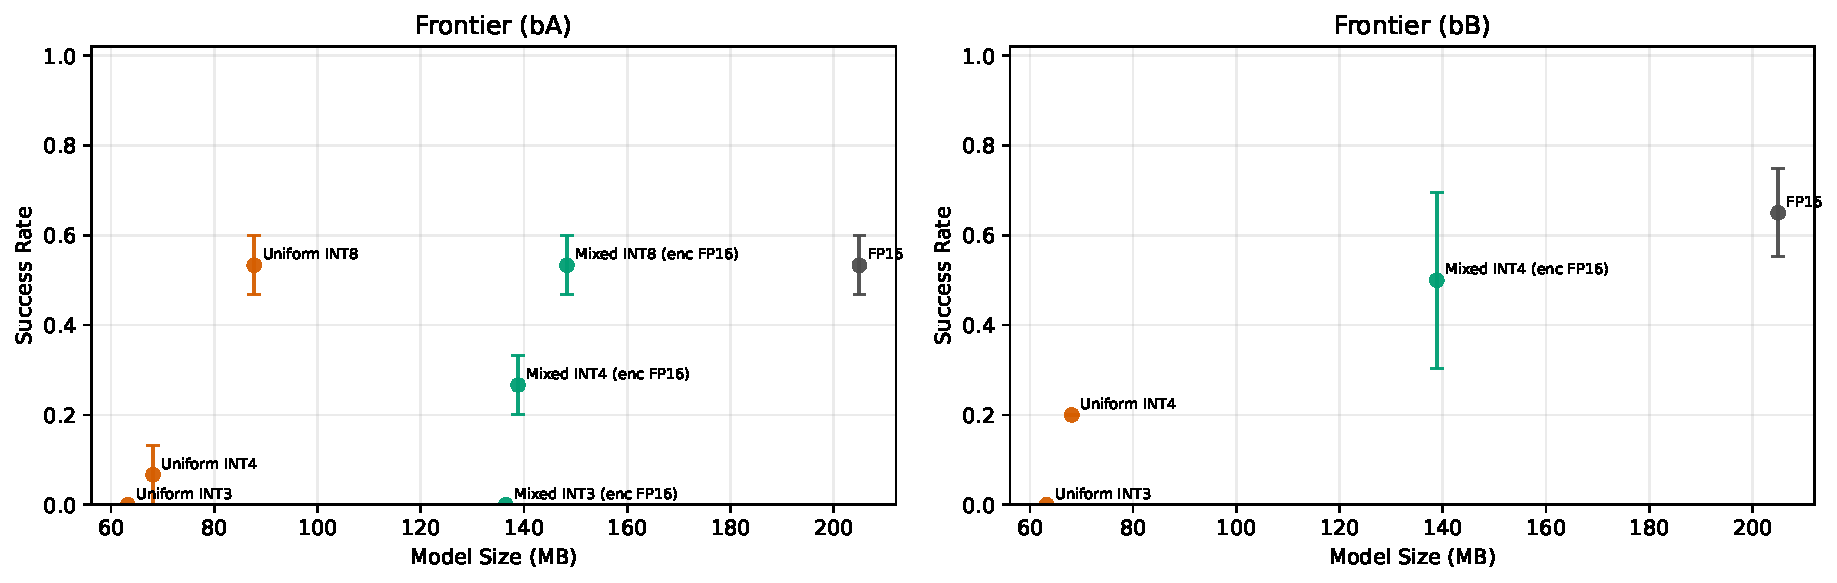
\includegraphics[width=0.98\linewidth]{../figures_transition/transition_run_v2/transition_frontier.pdf}
  \caption{Success--size frontier for core variants in the paired transition study. The 8-bit regime remains close to FP16, 3-bit variants collapse, and mixed INT4 stays above uniform INT4 in both budgets. Error bars are run-level 95\% confidence intervals.}
  \label{fig:frontier}
\end{figure}

\begin{figure}[t]
  \centering
  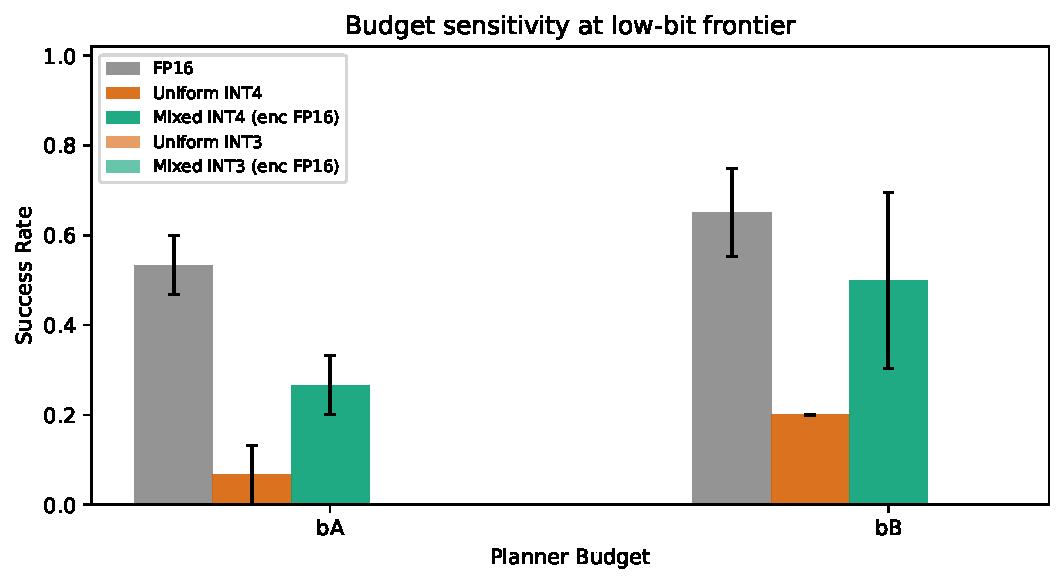
\includegraphics[width=0.98\linewidth]{../figures_transition/transition_run_v2/budget_sensitivity.pdf}
  \caption{Budget sensitivity across key variants. Increasing planner budget improves FP16 and INT4 variants, but does not recover uniform INT3; mixed INT4 remains consistently higher than uniform INT4.}
  \label{fig:budget}
\end{figure}

\begin{table}[t]
\centering
\small
\begin{tabular}{lcccc}
\toprule
Variant & Pilot & bA & bB & Size (MB) \\
\midrule
FP16 & 0.500 & 0.533 & 0.650 & 204.99 \\
Uniform INT8 & 0.500 & 0.533 & -- & 87.72 \\
Mixed INT8 & 0.500 & 0.533 & -- & 148.31 \\
Uniform INT4 & 0.083 & 0.067 & 0.200 & 68.12 \\
Mixed INT4 & \textbf{0.167} & \textbf{0.267} & \textbf{0.500} & 138.84 \\
Uniform INT3 & 0.000 & 0.000 & 0.000 & 63.23 \\
Mixed INT3 & 0.000 & 0.000 & -- & 136.47 \\
\bottomrule
\end{tabular}
\caption{Success-rate summary across runs and budgets. Pilot values come from the saved ten-variant sweep; bA/bB values come from the paired transition run.}
\label{tab:keyresults}
\end{table}

\section{Discussion and Open Questions}
The empirical pattern is clear enough to support a concrete research hypothesis: near the low-bit transition, preserving representation precision is more important than uniformly quantizing all modules.
At the same time, the mechanism is not fully resolved.
The budget sweep raises the first question: is the mixed-INT4 advantage mainly representational, or partly due to interaction with planner optimization depth?
Both INT4 variants improve with larger budget, but the mixed-uniform gap persists.
The layerwise sweep raises a second question: which encoder blocks are truly precision-critical, and are critical blocks task-dependent?
The non-monotonic intermediate points suggest this is not a simple ``more FP16 is always better'' effect.
The divergence diagnostics raise a third question: can explicit latent-geometry preservation objectives or calibration strategies close the uniform-INT4 gap without restoring full encoder precision?

\section{Limitations}
This is a single-environment study (Wall) with one pretrained checkpoint and moderate seed counts.
The paired confidence intervals for key deltas remain wide and include zero at this sample size.
We evaluate only weight-only quantization and do not test activation quantization, retraining, or hardware-fused low-bit kernels.
Therefore, the strongest claims are about robustness trends and module sensitivity under controlled settings, not universal optimality across tasks or hardware.

\section{Conclusion}
Across a pilot sweep and a larger paired transition study, DINO-WM planning shows a repeatable 8/4/3-bit phase structure and a consistent mixed-INT4 advantage over uniform INT4.
These results provide a concrete, testable direction for efficient spatial reasoning: design quantization policies that prioritize representation precision near low-bit operating frontiers.

\bibliography{references}
\bibliographystyle{iclr2026_conference}

\appendix
\clearpage
\section{Additional Results and Diagnostics}

\subsection{Paired Effect Estimates}
\begin{table}[h]
\centering
\small
\begin{tabular}{lcccccc}
\toprule
Budget & $n$ pairs & Mixed INT4 & Uniform INT4 & Delta & CI$_{95\%}$ (Delta) \\
\midrule
bA & 30 & 0.267 & 0.067 & +0.20 & [0.00, 0.40] \\
bB & 20 & 0.500 & 0.200 & +0.30 & [0.00, 0.55] \\
\bottomrule
\end{tabular}
\caption{Paired-goal mixed-vs-uniform INT4 deltas from transition\_run\_v2.}
\label{tab:paired}
\end{table}

\subsection{Transition-Run Summary Tables}
\begin{table}[h]
\centering
\small
\begin{tabular}{lcccc}
\toprule
Variant (bA) & Success & CI$_{95\%}$ & Time (s) & Size (MB) \\
\midrule
FP16 & 0.533 & [0.468, 0.599] & 49.66 & 204.99 \\
Uniform INT8 & 0.533 & [0.468, 0.599] & 50.44 & 87.72 \\
Mixed INT8 & 0.533 & [0.468, 0.599] & 48.29 & 148.31 \\
Uniform INT4 & 0.067 & [0.001, 0.132] & 46.54 & 68.12 \\
Mixed INT4 & 0.267 & [0.201, 0.332] & 48.36 & 138.84 \\
Uniform INT3 & 0.000 & [0.000, 0.000] & 41.10 & 63.23 \\
Mixed INT3 & 0.000 & [0.000, 0.000] & 41.53 & 136.47 \\
\bottomrule
\end{tabular}
\caption{Core transition-study results at budget bA (3 seeds).}
\label{tab:bAcore}
\end{table}

\begin{table}[h]
\centering
\small
\begin{tabular}{lcccc}
\toprule
Variant (bB) & Success & CI$_{95\%}$ & Time (s) & Size (MB) \\
\midrule
FP16 & 0.650 & [0.552, 0.748] & 124.45 & 204.99 \\
Uniform INT4 & 0.200 & [0.200, 0.200] & 130.05 & 68.12 \\
Mixed INT4 & 0.500 & [0.304, 0.696] & 141.44 & 138.84 \\
Uniform INT3 & 0.000 & [0.000, 0.000] & 135.27 & 63.23 \\
\bottomrule
\end{tabular}
\caption{Core transition-study results at budget bB (2 seeds).}
\label{tab:bBcore}
\end{table}

\begin{table}[h]
\centering
\small
\begin{tabular}{lccc}
\toprule
Encoder FP16 fraction & Success (bA) & CI$_{95\%}$ & Size (MB) \\
\midrule
0\%   & 0.10 & [0.100, 0.100] & 68.12 \\
25\%  & 0.05 & [0.000, 0.148] & 85.80 \\
50\%  & 0.15 & [0.052, 0.248] & 103.48 \\
75\%  & 0.05 & [0.000, 0.148] & 121.16 \\
100\% & 0.25 & [0.152, 0.348] & 138.84 \\
\bottomrule
\end{tabular}
\caption{INT4 encoder-retention ablation (predictor fixed at INT4, budget bA).}
\label{tab:layerwise}
\end{table}

\begin{table}[h]
\centering
\small
\begin{tabular}{lc}
\toprule
Metric vs Success & Spearman $\rho$ \\
\midrule
Mean state distance & -0.914 \\
Mean visual-embedding divergence & -0.779 \\
Mean proprio-embedding divergence & -0.710 \\
\bottomrule
\end{tabular}
\caption{Mechanistic correlations from transition\_run\_v2.}
\label{tab:mechcorr}
\end{table}

\begin{figure}[h]
  \centering
  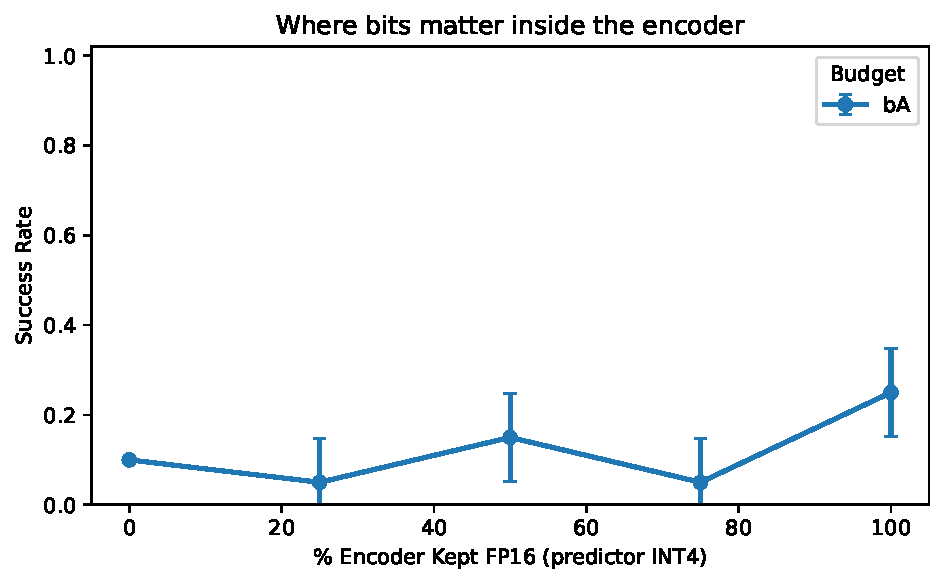
\includegraphics[width=0.95\linewidth]{../figures_transition/transition_run_v2/encoder_retention_curve.pdf}
  \caption{INT4 layerwise encoder-retention curve at budget bA. Keeping more encoder blocks in FP16 tends to improve success, with non-monotonic intermediate behavior.}
  \label{fig:enc_curve}
\end{figure}

\begin{figure}[h]
  \centering
  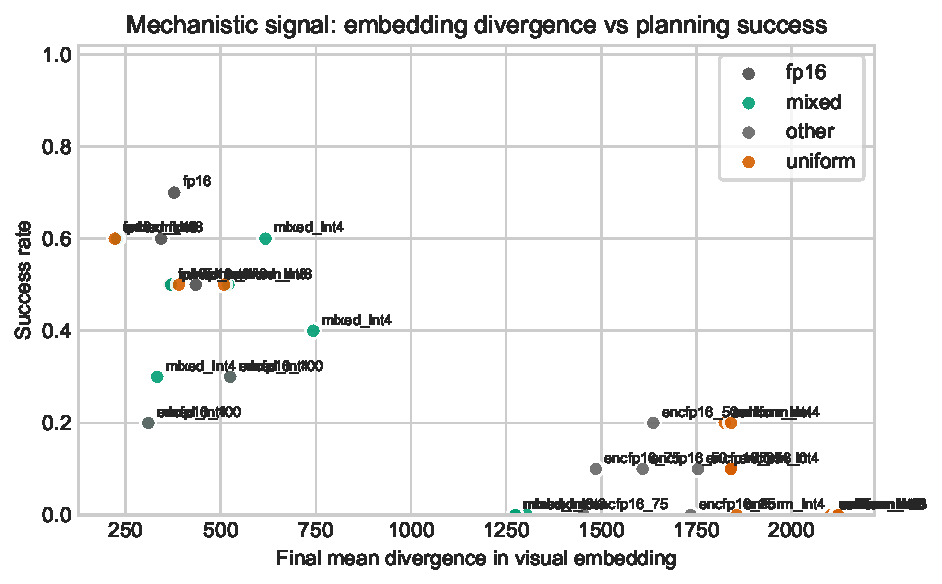
\includegraphics[width=0.95\linewidth]{../figures_transition/transition_run_v2/mechanistic_success_vs_divergence.pdf}
  \caption{Mechanistic diagnostic: variants with higher visual-embedding divergence tend to have lower planning success.}
  \label{fig:mech}
\end{figure}

\begin{figure}[h]
  \centering
  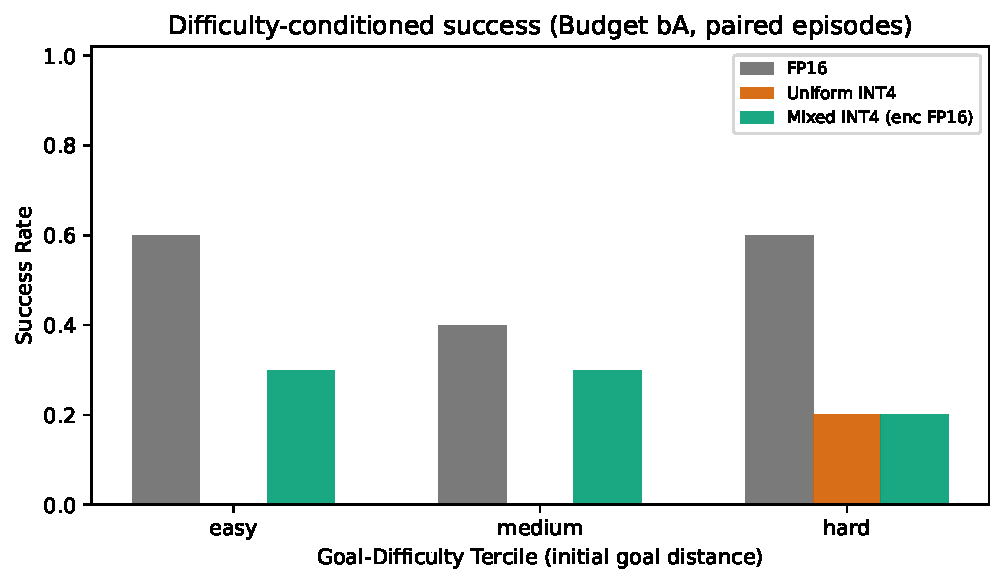
\includegraphics[width=0.95\linewidth]{../figures_transition/transition_run_v2/difficulty_conditioned_success.pdf}
  \caption{Difficulty-conditioned success in budget bA (difficulty terciles from initial goal distance). Uniform INT4 is brittle across bins; mixed INT4 improves success across bins relative to uniform INT4.}
  \label{fig:difficulty}
\end{figure}

\clearpage
\subsection{Pilot-Run Replication Figures (Saved Snapshot)}
\begin{figure}[h]
  \centering
  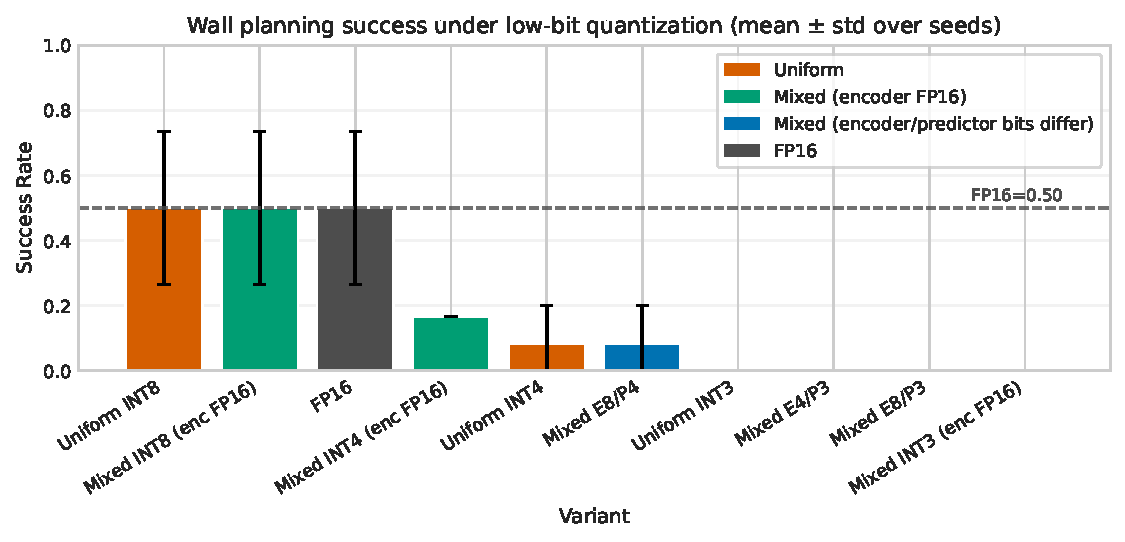
\includegraphics[width=0.95\linewidth]{../figures_bitsweep_h9_mixed/bitsweep_success_bars.pdf}
  \caption{Pilot ten-variant sweep (saved snapshot). This run first exposed the same 8/4/3-bit phase pattern later revalidated in the paired transition study.}
  \label{fig:pilotbars}
\end{figure}

\begin{figure}[h]
  \centering
  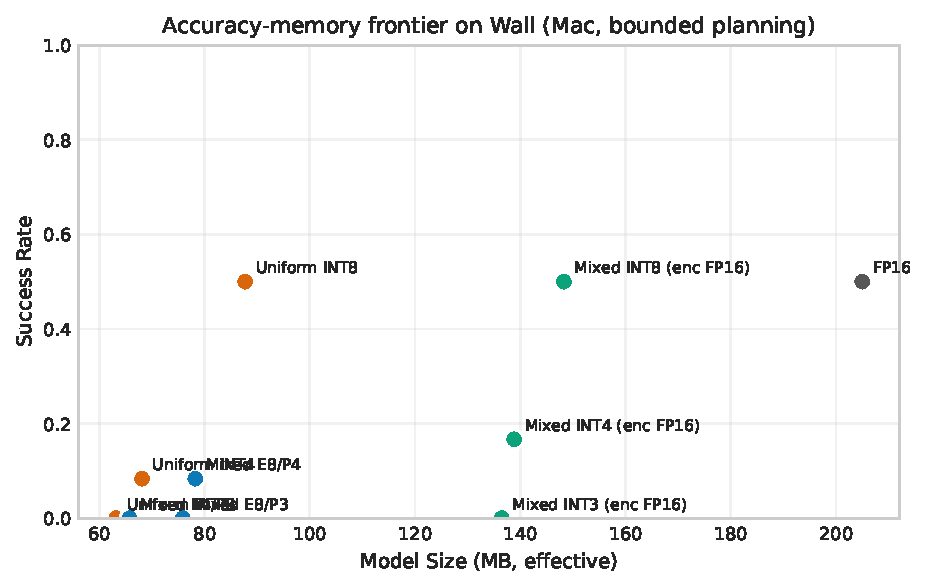
\includegraphics[width=0.95\linewidth]{../figures_bitsweep_h9_mixed/bitsweep_frontier.pdf}
  \caption{Pilot success--size frontier over ten variants. Mixed INT4 is above uniform INT4 while 3-bit variants collapse.}
  \label{fig:pilotfrontier}
\end{figure}

\end{document}
